\documentclass[a4paper,12pt]{article}
\usepackage[utf8]{inputenc}
\usepackage{graphicx}
\usepackage{float}
\usepackage[spanish]{babel}
\usepackage{listings}
\usepackage{xcolor}
\usepackage{courier}
\usepackage[T1]{fontenc}

\definecolor{gris}{RGB}{123, 126, 132}
\definecolor{morado}{RGB}{81, 40, 155}
\definecolor{amarillo}{RGB}{253,151,31}
\definecolor{magenta}{RGB}{249,38,114}

\renewcommand{\lstlistingname}{Archivo}

\lstdefinestyle{customJava}{
    frame=tb,
    language=Java,
    backgroundcolor=\color{white},   
    commentstyle=\itshape\color{gris},
    keywordstyle=\bfseries\color{magenta},
    numberstyle=\color{morado},
    stringstyle=\color{amarillo},
    identifierstyle=\color{black},
    basicstyle=\footnotesize,
    breakatwhitespace=false,         
    breaklines=true,                 
    captionpos=b,
    keepspaces=true,                 
    numbers=left,                    
    numbersep=5pt,                  
    showspaces=false,                
    showstringspaces=false,
    showtabs=false,                  
    tabsize=2,
}

\lstdefinestyle{customXML}{
    frame=tb,
    language=XML,
    backgroundcolor=\color{white},   
    commentstyle=\itshape\color{gris},
    keywordstyle=\bfseries\color{magenta},
    numberstyle=\color{morado},
    stringstyle=\color{amarillo},
    identifierstyle=\color{black},
    basicstyle=\footnotesize,
    breakatwhitespace=false,         
    breaklines=true,                 
    captionpos=b,
    keepspaces=true,                 
    numbers=left,                    
    numbersep=5pt,                  
    showspaces=false,                
    showstringspaces=false,
    showtabs=false,                  
    tabsize=2,
}

%opening
\title{Ejercicio No. 5. Categoria-Producto (Consola)}
\author{Barrera Pérez Carlos Tonatihu \\ Profesor: José Asunción Enríquez 
Zárate \\ Web Application Development \\ Grupo: 3CM9 }

\begin{document}

\maketitle

\newpage
\tableofcontents
\newpage
\section{Introducción}
Este ejercicio tuvo como objetivo desarrollar un pequeño CRUD para la base de 
datos que se muestra en la figura \ref{fig:bd}.

\begin{figure}[H]
\begin{center}
 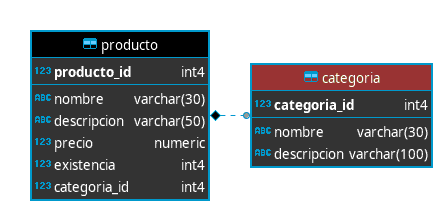
\includegraphics[width=\textwidth]{bd.png}
 \caption{Base de datos que se trabajo en PostgreSQL}
 \label{fig:bd}
\end{center}
\end{figure}

A diferencia del CRUD en consola que se realizo con anterioridad, en este se 
utilizo Hibernate para agilizar el acceso a datos. Y de nueva cuenta se utilizo 
el patrón DAO para realizar una implementación que no generara problemas en un 
futuro. 

\section{Desarrollo}

\subsection{Código}
Las siguientes dos secciones de código se utilizan para configurar Hibernate y 
poder conectarse a la base de datos.

\begin{lstlisting}[language=XML, style=customXML, 
caption={hibernate.cfg.xml}, captionpos=b,basicstyle=\fontfamily{cmss}\small]
<?xml version="1.0" encoding="UTF-8"?>
<!DOCTYPE hibernate-configuration PUBLIC
        "-//Hibernate/Hibernate Configuration DTD//EN"
        "http://www.hibernate.org/dtd/hibernate-configuration-3.0.dtd">
<hibernate-configuration>
  <session-factory>
    <property 
name="hibernate.dialect">org.hibernate.dialect.PostgreSQLDialect</property>
    <property 
name="hibernate.connection.driver_class">org.postgresql.Driver</property>
    <property 
name="hibernate.connection.url">jdbc:postgresql://localhost:5432/tiendita</prope
rty>
    <property name="hibernate.connection.username">postgres</property>
    <property name="connection.password">respuesta42</property>
    <property name="show_sql">true</property>
        <property name="format_sql">true</property>
    <property name="hibernate.current_session_context_class">thread</property>
    
    <mapping class="tiendita.entity.CategoriaEntity"/>
    <mapping class="tiendita.entity.ProductoEntity"/>
  </session-factory>
</hibernate-configuration>
\end{lstlisting}

\begin{lstlisting}[language=Java, style=customJava, 
caption={HibernateUtil.java}, captionpos=b,basicstyle=\fontfamily{cmss}\small]
package tiendita.util;

import org.hibernate.HibernateException;
import org.hibernate.Session;
import org.hibernate.SessionFactory;
import org.hibernate.cfg.Configuration;

/**
 * Hibernate Utility class with a convenient method to get Session Factory
 * object.
 *
 * @author tonatihu
 */
public class HibernateUtil {
    private static final SessionFactory ourSessionFactory;

    static {
        try {
            Configuration configuration = new Configuration();
            configuration.configure();

            ourSessionFactory = configuration.buildSessionFactory();
        } catch (HibernateException ex) {
            throw new ExceptionInInitializerError(ex);
        }
    }

    public static Session getSession() throws HibernateException {
        return ourSessionFactory.openSession();
    }
}
\end{lstlisting}

A continuación se muestran las entidades que se configuraron en el archivo de 
configuración y que mapean las tablas que se encuentran en la base de datos.

\begin{lstlisting}[language=Java, style=customJava, 
caption={CategoriaEntity.java}, captionpos=b,basicstyle=\fontfamily{cmss}\small]
package tiendita.entity;

import java.io.Serializable;
import java.util.ArrayList;
import java.util.List;
import java.util.Objects;
import javax.persistence.Basic;
import javax.persistence.Column;
import javax.persistence.Entity;
import javax.persistence.GeneratedValue;
import javax.persistence.GenerationType;
import javax.persistence.Id;
import javax.persistence.OneToMany;
import javax.persistence.Table;

/**
 *
 * @author tonatihu
 * Created on 02-Jun-2019
 */
@Entity
@Table(name = "categoria", schema = "public", catalog = "tiendita")
public class CategoriaEntity implements Serializable {
    @Id
    @GeneratedValue(strategy = GenerationType.IDENTITY)
    @Column(name = "categoria_id", nullable = false)
    private int categoriaId;
    @Basic
    @Column(name = "nombre", nullable = false, length = 30)
    private String nombre;
    @Basic
    @Column(name = "descripcion", nullable = false, length = 100)
    private String descripcion;

    @OneToMany(mappedBy = "categoria")
    private List<ProductoEntity> productos = new ArrayList<>();

    public int getCategoriaId() {
        return categoriaId;
    }

    public void setCategoriaId(int categoriaId) {
        this.categoriaId = categoriaId;
    }

    public String getNombre() {
        return nombre;
    }

    public void setNombre(String nombre) {
        this.nombre = nombre;
    }

    public String getDescripcion() {
        return descripcion;
    }

    public void setDescripcion(String descripcion) {
        this.descripcion = descripcion;
    }


    public List<ProductoEntity> getProductos() {
        return productos;
    }

    public void setProductos(List<ProductoEntity> productos) {
        this.productos = productos;
    }

    public void addProducto(ProductoEntity producto) {
        this.productos.add(producto);
    }

    @Override
    public boolean equals(Object o) {
        if (this == o) return true;
        if (o == null || getClass() != o.getClass()) return false;
        CategoriaEntity that = (CategoriaEntity) o;
        return categoriaId == that.categoriaId && Objects.equals(nombre, 
that.nombre) &&
                Objects.equals(descripcion, that.descripcion);
    }

    @Override
    public int hashCode() {
        return Objects.hash(categoriaId, nombre, descripcion);
    }

    @Override
    public String toString() {
        return "CategoriaEntity{" + "categoriaId=" + categoriaId + ", nombre='" 
+ nombre + '\'' +
                ", descripcion='" + descripcion + '\'' + '}';
    }
}
\end{lstlisting}

\begin{lstlisting}[language=Java, style=customJava, 
caption={ProductoEntity.java}, captionpos=b,basicstyle=\fontfamily{cmss}\small]
package tiendita.entity;

import java.io.Serializable;
import java.math.BigDecimal;
import java.util.Objects;
import javax.persistence.Basic;
import javax.persistence.Column;
import javax.persistence.Entity;
import javax.persistence.GeneratedValue;
import javax.persistence.GenerationType;
import javax.persistence.Id;
import javax.persistence.JoinColumn;
import javax.persistence.ManyToOne;
import javax.persistence.Table;

/**
 *
 * @author tonatihu
 * Created on 02-Jun-2019
 */
@Entity
@Table(name = "producto", schema = "public", catalog = "tiendita")
public class ProductoEntity implements Serializable {
    @Id
    @GeneratedValue(strategy = GenerationType.IDENTITY)
    @Column(name = "producto_id", nullable = false)
    private int productoId;
    @Basic
    @Column(name = "nombre", nullable = false, length = 30)
    private String nombre;
    @Basic
    @Column(name = "descripcion", nullable = false, length = 50)
    private String descripcion;
    @Basic
    @Column(name = "precio", nullable = false)
    private BigDecimal precio;
    @Basic
    @Column(name = "existencia", nullable = false)
    private int existencia;

    @ManyToOne
    @JoinColumn(name = "categoria_id", referencedColumnName = "categoria_id", 
nullable = false)
    private CategoriaEntity categoria;


    public int getProductoId() {
        return productoId;
    }

    public void setProductoId(int productoId) {
        this.productoId = productoId;
    }

    public String getNombre() {
        return nombre;
    }

    public void setNombre(String nombre) {
        this.nombre = nombre;
    }

    public String getDescripcion() {
        return descripcion;
    }

    public void setDescripcion(String descripcion) {
        this.descripcion = descripcion;
    }

    public BigDecimal getPrecio() {
        return precio;
    }

    public void setPrecio(BigDecimal precio) {
        this.precio = precio;
    }

    public int getExistencia() {
        return existencia;
    }

    public void setExistencia(int existencia) {
        this.existencia = existencia;
    }

    @Override
    public boolean equals(Object o) {
        if (this == o) return true;
        if (o == null || getClass() != o.getClass()) return false;
        ProductoEntity that = (ProductoEntity) o;
        return productoId == that.productoId && existencia == that.existencia && 
Objects.equals(
                nombre, that.nombre) && Objects.equals(descripcion, 
that.descripcion) &&
                Objects.equals(precio, that.precio);
    }

    @Override
    public int hashCode() {
        return Objects.hash(productoId, nombre, descripcion, precio, 
existencia);
    }

    public CategoriaEntity getCategoria() {
        return categoria;
    }

    public void setCategoria(CategoriaEntity categoria) {
        this.categoria = categoria;
    }

    @Override
    public String toString() {
        return "ProductoEntity{" + "productoId=" + productoId + ", nombre='" + 
nombre + '\'' +
                ", descripcion='" + descripcion + '\'' + ", precio=" + precio + 
", existencia=" +
                existencia + ", categoria=" + categoria + '}';
    }
}
\end{lstlisting}

La siguientes tres secciones de código es la implementación del patrón DAO, 
utilizando primero una clase abstracta que modela el comportamiento del resto 
de DAOs.

\begin{lstlisting}[language=Java, style=customJava, 
caption={GenericDAO.java}, captionpos=b,basicstyle=\fontfamily{cmss}\small]

package dao;

import java.io.Serializable;
import java.util.List;
import org.hibernate.Session;
import org.hibernate.Transaction;
import tiendita.util.HibernateUtil;

/**
 *
 * @author tonatihu
 * Created on 02-Jun-2019
 */
public abstract class GenericDAO <T, Id extends Serializable>{
    private Session currentSession;
    private Transaction currentTransaction;

    public void openCurrentSession() {
        currentSession = HibernateUtil.getSession();
    }

    public void openCurrentSessionWithTransaction() {
        currentSession = HibernateUtil.getSession();
        currentTransaction = currentSession.beginTransaction();
    }

    public void closeCurrentSession() {
        currentSession.close();
    }

    public void closeCurrentSessionwithTransaction() {
        currentTransaction.commit();
        currentSession.close();
    }

    public void rollback() {
        if (currentTransaction != null)
            currentTransaction.rollback();
    }

    protected Session getCurrentSession() {
        return currentSession;
    }

    public abstract void create(T entity);
    public abstract void update(T entity);
    public abstract T findById(Id id);
    public abstract void delete(T entity);
    public abstract List<T> findAll();
}


\end{lstlisting}

\begin{lstlisting}[language=Java, style=customJava, 
caption={CategoriaDAOImpl.java}, 
captionpos=b,basicstyle=\fontfamily{cmss}\small]
package dao.impl;

import dao.GenericDAO;
import java.util.List;
import java.util.logging.Level;
import java.util.logging.Logger;
import org.hibernate.HibernateException;
import tiendita.entity.CategoriaEntity;

/**
 *
 * @author tonatihu
 * Created on 02-Jun-2019
 */
public class CategoriaDAOImpl extends GenericDAO<CategoriaEntity, Integer> {
    private static final Logger LOGGER = Logger
            .getLogger(CategoriaDAOImpl.class.getName());
    @Override
    public void create(CategoriaEntity entity) {
        openCurrentSessionWithTransaction();
        try {
            getCurrentSession().save(entity);
        } catch (HibernateException hehe) {
            LOGGER.log(Level.SEVERE, "Error en create", hehe);
            rollback();
        } finally {
            closeCurrentSessionwithTransaction();
        }
    }

    @Override
    public void update(CategoriaEntity entity) {
        openCurrentSessionWithTransaction();
        try {
            getCurrentSession().update(entity);
        } catch (HibernateException hehe) {
            LOGGER.log(Level.SEVERE, "Error en update", hehe);
            rollback();
        } finally {
            closeCurrentSessionwithTransaction();
        }
    }

    @Override
    public CategoriaEntity findById(Integer integer) {
        openCurrentSession();
        CategoriaEntity categoriaEntity = (CategoriaEntity) getCurrentSession()
                .get(CategoriaEntity.class, integer);
        closeCurrentSession();
        return categoriaEntity;
    }

    @Override
    public void delete(CategoriaEntity entity) {
        openCurrentSessionWithTransaction();
        try {
            getCurrentSession().delete(entity);
        } catch (HibernateException hehe) {
            LOGGER.log(Level.SEVERE, "Error en delete", hehe);
            rollback();
        } finally {
            closeCurrentSessionwithTransaction();
        }
    }

    @Override
    @SuppressWarnings("unchecked")
    public List<CategoriaEntity> findAll() {
        openCurrentSession();
        List<CategoriaEntity> lista = (List<CategoriaEntity>) 
getCurrentSession()
                .createQuery("from CategoriaEntity").list();
        closeCurrentSession();
        return lista;
    }
}
\end{lstlisting}

\begin{lstlisting}[language=Java, style=customJava, 
caption={ProductoDAOImpl.java}, captionpos=b,basicstyle=\fontfamily{cmss}\small]
package dao.impl;

import dao.GenericDAO;
import java.util.List;
import java.util.logging.Level;
import java.util.logging.Logger;
import org.hibernate.HibernateException;
import tiendita.entity.ProductoEntity;

/**
 *
 * @author tonatihu
 * Created on 02-Jun-2019
 */
public class ProductoDAOImpl extends GenericDAO<ProductoEntity, Integer> {
    private static final Logger LOGGER = Logger
            .getLogger(ProductoDAOImpl.class.getName());
    @Override
    public void create(ProductoEntity entity) {
        openCurrentSessionWithTransaction();
        try {
            getCurrentSession().save(entity);
        } catch (HibernateException hehe) {
            LOGGER.log(Level.SEVERE, "Error en create", hehe);
            rollback();
        } finally {
            closeCurrentSessionwithTransaction();
        }
    }

    @Override
    public void update(ProductoEntity entity) {
        openCurrentSessionWithTransaction();
        try {
            getCurrentSession().update(entity);
        } catch (HibernateException hehe) {
            LOGGER.log(Level.SEVERE, "Error en update", hehe);
            rollback();
        } finally {
            closeCurrentSessionwithTransaction();
        }
    }

    @Override
    public ProductoEntity findById(Integer integer) {
        openCurrentSession();
        ProductoEntity productoEntity = (ProductoEntity) getCurrentSession()
                .get(ProductoEntity.class, integer);
        closeCurrentSession();
        return productoEntity;
    }

    @Override
    public void delete(ProductoEntity entity) {
        openCurrentSessionWithTransaction();
        try {
            getCurrentSession().delete(entity);
        } catch (HibernateException hehe) {
            LOGGER.log(Level.SEVERE, "Error en delete", hehe);
            rollback();
        } finally {
            closeCurrentSessionwithTransaction();
        }
    }

    @Override
    @SuppressWarnings("unchecked")
    public List<ProductoEntity> findAll() {
        openCurrentSession();
        List<ProductoEntity> lista = (List<ProductoEntity>) getCurrentSession()
                .createQuery("from ProductoEntity").list();
        closeCurrentSession();
        return lista;
    }
}

\end{lstlisting}

Finalmente se tiene la clase principal en donde se trabajó el CRUD y se utilizo 
todo lo anterior.

\begin{lstlisting}[language=Java, style=customJava, 
caption={Tiendita.java}, captionpos=b,basicstyle=\fontfamily{cmss}\small]
package tiendita;

import dao.impl.CategoriaDAOImpl;
import java.io.BufferedReader;
import java.io.IOException;
import java.io.InputStreamReader;
import java.util.List;
import tiendita.entity.CategoriaEntity;

/**
 *
 * @author tonatihu
 * Created on 02-Jun-2019
 */
public class Tiendita {

    /**
     * @param args the command line arguments
     * @throws java.io.IOException
     */
   public static void main(String[] args) throws IOException {
        boolean continuar = true;
        int opcion = 0;
        BufferedReader br = new BufferedReader(new 
InputStreamReader(System.in));
        CategoriaDAOImpl dao = new CategoriaDAOImpl();
        CategoriaEntity categoria;

        while (continuar) {
            System.out.println("1) Alta categoria");
            System.out.println("2) Baja categoria");
            System.out.println("3) Cambio categoria");
            System.out.println("4) Consultar categoria");
            System.out.println("5) Consultar todas las categorias");
            System.out.println("6) Salir");
            System.out.println("Selecciona una opcion:");
            opcion = Integer.valueOf(br.readLine());
            switch(opcion) {
                case 1: // alta
                    System.out.println("ALTA");
                    categoria = new CategoriaEntity();
                    System.out.println("Ingrese el nombre:");
                    categoria.setNombre(br.readLine());
                    System.out.println("Ingrese la descripcion:");
                    categoria.setDescripcion(br.readLine());
                    dao.create(categoria);
                    System.out.println("Listo...");
                    break;
                case 2: // baja
                    System.out.println("BAJA");
                    categoria = new CategoriaEntity();
                    System.out.println("Ingrese el id:");
                    categoria.setCategoriaId(Integer.valueOf(br.readLine()));
                    categoria = dao.findById(categoria.getCategoriaId());
                    dao.delete(categoria);
                    System.out.println("Listo...");
                    break;
                case 3: // cambio
                    System.out.println("CAMBIO");
                    categoria = new CategoriaEntity();
                    System.out.println("Ingrese el id:");
                    categoria.setCategoriaId(Integer.valueOf(br.readLine()));
                    System.out.println("Ingrese la descripcion:");
                    categoria.setDescripcion(br.readLine());
                    System.out.println("Ingrese el nombre:");
                    categoria.setNombre(br.readLine());
                    System.out.println("Listo...");
                    dao.update(categoria);
                    break;
                case 4: // consulta
                    System.out.println("CONSULTA");
                    categoria = new CategoriaEntity();
                    System.out.println("Ingrese el id:");
                    categoria.setCategoriaId(Integer.valueOf(br.readLine()));
                    categoria = dao.findById(categoria.getCategoriaId());
                    if (categoria != null)
                        System.out.println(categoria.toString());
                    System.out.println("Listo...");
                    break;
                case 5: // consulta todos
                    System.out.println("CONSULTAR TODOS");
                    List<CategoriaEntity> categorias = dao.findAll();
                    for (CategoriaEntity c : categorias) {
                        System.out.println(c.toString());
                    }
                    System.out.println("Listo");
                    break;
                default:
                    continuar = false;
                    break;
            }
        }
        System.out.println("See you space cowboy...");
    }
}
\end{lstlisting}

\subsection{Consultar todos}
\begin{figure}[H]
\begin{center}
 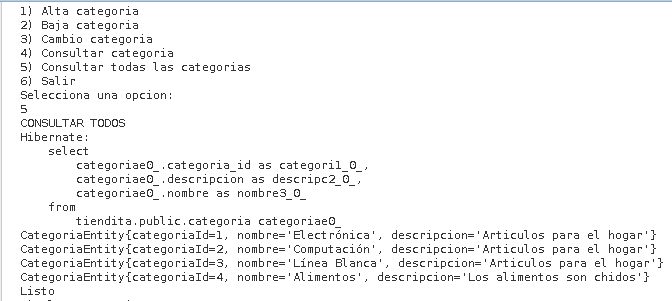
\includegraphics[width=\textwidth]{consultar_todos.png}
 \caption{Se consultan todos}
 \label{fig:todos}
\end{center}
\end{figure}

\subsection{Cambio}
\begin{figure}[H]
\begin{center}
 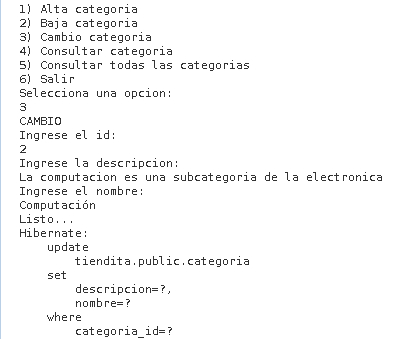
\includegraphics[width=\textwidth]{cambio.png}
 \caption{Se realizan cambios en una categoría}
 \label{fig:cambio}
\end{center}
\end{figure}

\subsection{Consulta}
\begin{figure}[H]
\begin{center}
 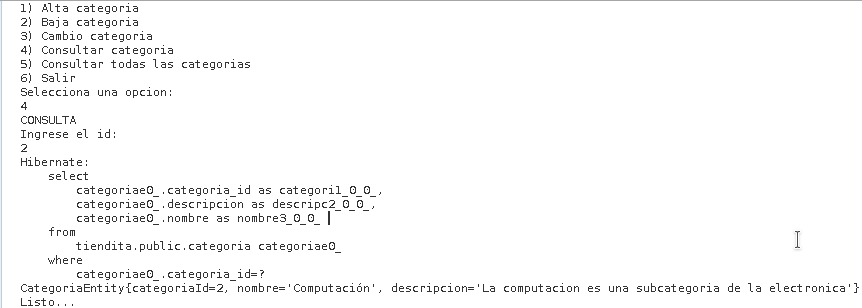
\includegraphics[width=\textwidth]{consulta.png}
 \caption{Se realiza una consulta en el que se realizo el cambio}
 \label{fig:consulta}
\end{center}
\end{figure}

\subsection{Alta}
\begin{figure}[H]
\begin{center}
 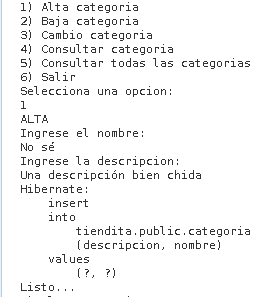
\includegraphics[width=\textwidth]{alta.png}
 \caption{Alta de una categoría}
 \label{fig:alta}
\end{center}
\end{figure}

\subsection{Baja}
\begin{figure}[H]
\begin{center}
 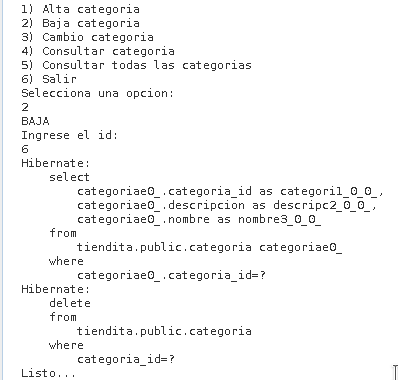
\includegraphics[width=\textwidth]{baja.png}
 \caption{Baja de una categoría}
 \label{fig:alta}
\end{center}
\end{figure}

\section{Conclusiones}
El uso de Hibernate facilita bastante el trabajar con bases de datos ya que se 
pueden evitar bastantes pasos que se tenían que realizar usando solamente JDBC 
como es el caso de la conexión a la base de datos.

Es importante tener en cuenta que se debe de usar correctamente ya que de lo 
contrario podría generar más problemas de los que pretende solucionar. En este 
caso, debido a el como se implemento puede ser usado en futuros trabajos de 
esta materia ya que el uso de Hibernate no se restringe solo a proyectos web o 
hechos solo con Java.

\end{document}
